\documentclass[utf8]{article}
\usepackage[utf8]{inputenc}
\usepackage[french]{babel}
\usepackage{amsmath}
\usepackage{amsthm}
\usepackage[pdftex]{graphicx}
\title{Rapport d'avancement 3ème année}
\newtheorem{The}{Théorème}
\author{Martin Averseng}
\begin{document}
	\maketitle
	
	\section{Mois de soutenance et formations suivies}
	
	Formations complémentaires suivies : 
	\begin{itemize}
		\item[-] Organisation du spectacle Pi Day en 2016, un événement qui a rassemblé plus de 1500 spectateurs français de différentes villes autour de la diffusion scientifique, pour un total de 28 heures de formation.
		\item[-] Participation au séminaire des doctorants et présentation de mon travail aux autres doctorants, valant 12 heures de formation. 
		\item[-] Journée EDP-neurosciences de la SMAI, 4 heures
		\item[-] Participation au stand Fab-Maths lors de la fête de la science, 7 heures de formation.  
	\end{itemize}
	
	Il me manque donc à ce jour 5 heures de formation que je terminerai au cours de cette année. Par ailleurs, la soutenance de la thèse est prévue entre Septembre et Novembre 2019. 
	
	\section{Travail accompli en 2ème année}
	
	La deuxième année de cette thèse à été consacrée à la mise en œuvre et l'analyse d'une nouvelle méthode de résolution d'équations intégrales dans le plan sur des courbes ouvertes.
	
	\subsection{Equations intégrales sur des courbes ouvertes}
	
	Le problème des équations intégrales sur une courbe ouverte est double. D'abord, les singularités géométriques au bord de la courbe mènent à des solutions singulières. La résolution numérique habituelle utilisant des fonctions polynomiales par morceaux échoue à capturer ce comportement singulier, ce qui se traduit par une faible vitesse de convergence en fonction du pas $h$ du maillage. Il faut donc utiliser d'autres méthodes pour discrétiser ces équations, qui mènent à une convergence plus rapide. De nombreuses possibilités existent : ajouter dans l'espace d'approximation les fonctions singulières explicitement connues, raffiner le maillage près des singularités, etc.
	
	Le deuxième problème est alors le choix du préconditionneur pour le nouveau système linéaire obtenu car les méthodes habituelles ne sont généralement plus valides dans ce cas. Par exemple, une des méthodes en l'absence de singularités géométriques est d'utiliser le calcul pseudo-différentiel sur le bord de l'objet, trouver le symbole principal de l'opérateur et construire grâce à cela une paramétrix que l'on discrétise ensuite pour l'utiliser comme un préconditionneur. Cette méthode est impossible dans le cas d'une courbe ouverte sur laquelle on n'a pas de notion de calcul pseudo-différentiel. 
	
	\subsection{Méthode de Galerkin à poids}
	
	L'approche que nous avons suivie cette année est la suivante. Supposons que l'on cherche à résoudre l'équation $S \lambda  = u_0$ d'inconnue $\lambda$ définie sur la courbe ouverte $\Gamma$. Si $u_0$ est régulière, dans notre contexte, on sait que $\lambda$ s'écrit come $\frac{\alpha}{\omega}$ où $\omega$ est une fonction explicite de "poids" qui s'annule aux bords de $\Gamma$, capturant ainsi la singularité de $\lambda$, tandis que $\alpha$ est régulière. On résout alors $S_\omega\alpha := S\frac{1}{\omega} \alpha = u_0$ d'inconnue $\alpha$. Si l'on résout numériquement cette équation par une méthode de Galerkin avec des fonctions affines par morceaux, nous avons prouvé que l'on retrouve l'ordre de convergence habituel dans le cas d'une courbe régulière. 
	\begin{The}
		Si $u$ est suffisamment régulière, alors la solution $\alpha_h$ de la mé\-thode variationnelle pour un maillage de pas $h$ converge vers la vraie solution $\alpha$ avec 
		\[\|\alpha - \alpha_h\| \leq C h^{5/2} \,.\]
	\end{The}
	
	\subsection{Nouveaux préconditionneurs}
	
	Dans un deuxième temps, une fois que la méthode numérique possède ces bonnes propriétés de convergence, on cherche à proposer un préconditionneur efficace pour le système linéaire. Après avoir remarqué que l'opérateur $S_\omega$ commutait avec l'opérateur $(\omega \partial_x)^2 + k^2\omega^2$, nous avons émit la conjecture selon laquelle 
	\[\sqrt{-(\omega \partial_x)^2 - k^2\omega^2} S_\omega = I_d + K\]
	où $K$ est un opérateur compact. Cette formule est en analogie frappante avec les préconditionneurs issus de l'analyse pseudo-différentielle dans le cas des courbes régulières. Dans ce cas, on a en effet
	\[\sqrt{-(\partial_x)^2 - k^2} S = I_d + K\]
	c'est-à-dire la même formule avec $\omega = 1$. 
	
	\subsubsection{Mise en œuvre numérique}
	
	J'ai construit un code Matlab d'équations intégrales en 2D permettant de tester cette hypothèse. Ce code utilise la méthode de compression et d'accélération des convolutions discrètes développé en stage pré-thèse. Il implémente les diffé\-rents opérateurs intégraux à poids que nous étudions, et la méthode de Galerkin à poids décrite précédemment. Il a permis de confirmer les performances excellentes du préconditionneur proposé ci-dessus. Voici un exemple des possibilités offertes par ce code.
	
	\begin{figure}[h]
		\centering
		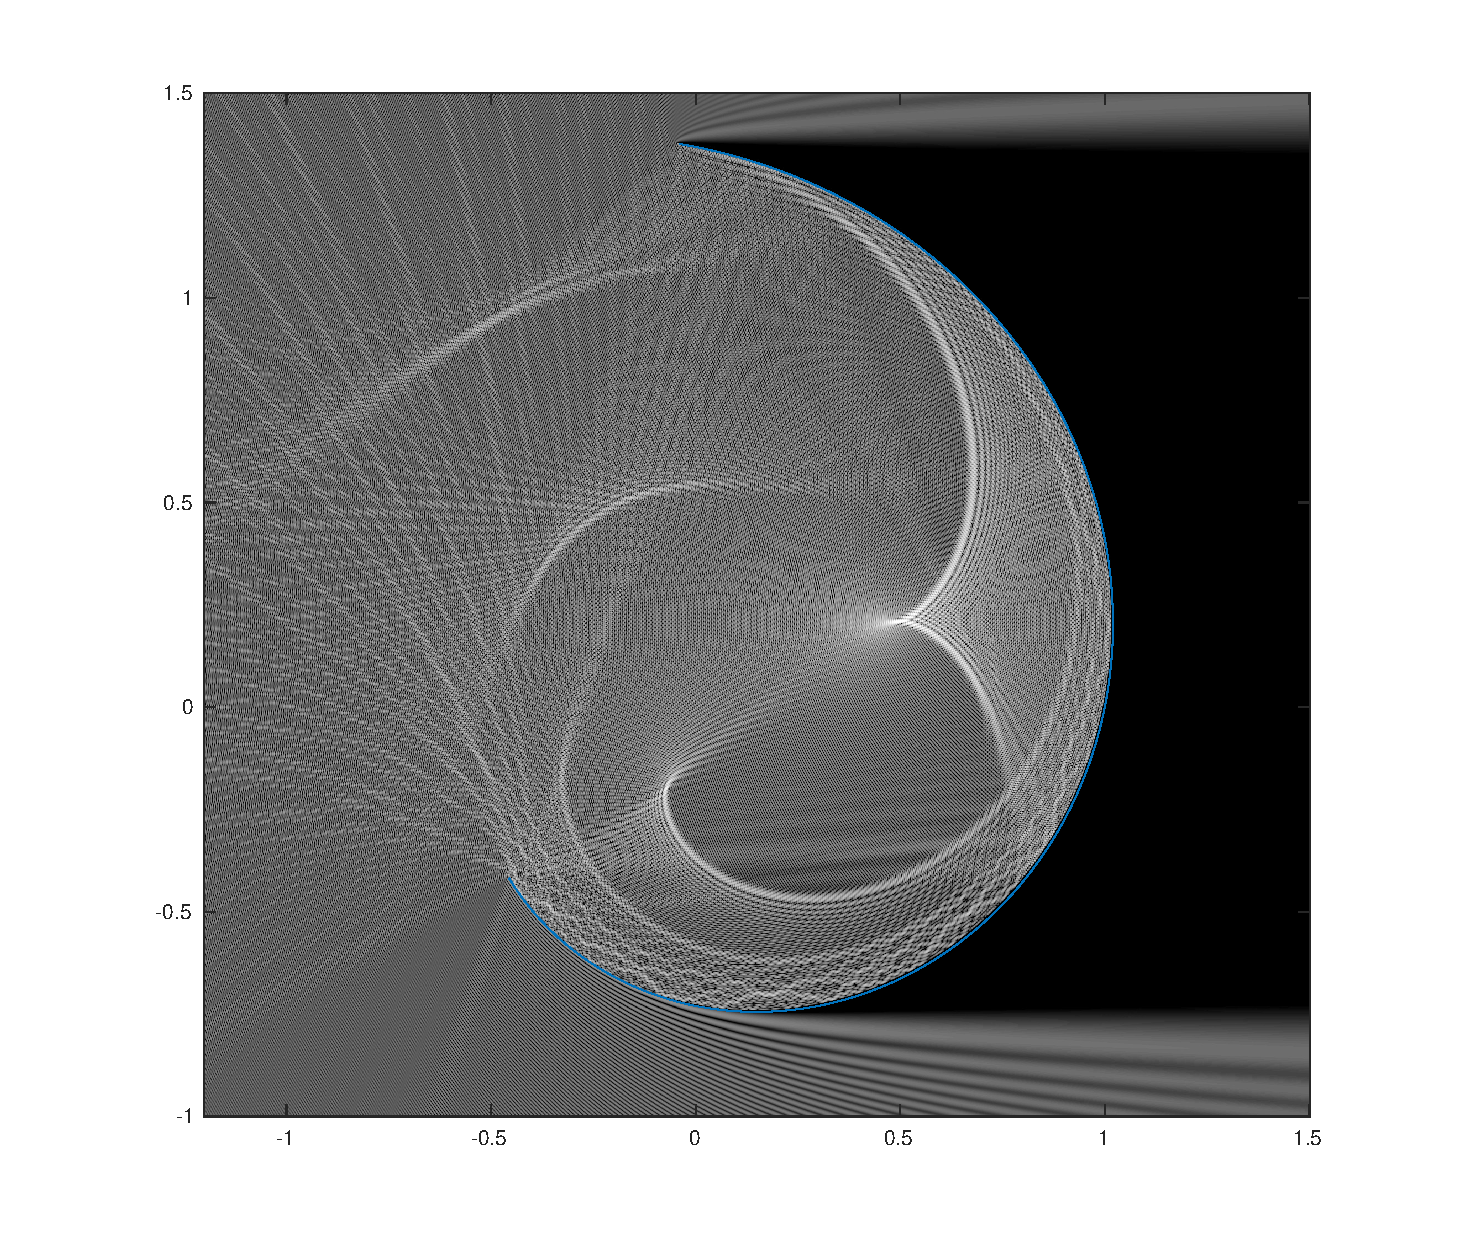
\includegraphics[scale = 0.2]{arcOfSpiral800_3}
		\caption{Diffraction par un arc de spirale. }
	\end{figure}

	\subsubsection{Analyse pseudo-différentielle}

	Pour confirmer théoriquement les performances de ces préconditionneurs, nous avons développé un outil de calcul pseudo-différentiel sur des courbes ouvertes. Cela nous a permis de prouver la conjecture. À notre connaissance, rien de comparable n'existe dans la littérature. 
	
	\begin{The}
		Il existe un opérateur compact $K$ tel que
		\[\sqrt{-(\omega \partial_x)^2 - k^2 \omega^2} S_\omega = I_d + K\]
	\end{The}
	
	\subsection{Publication}
	
	Ces idées seront soumises sous la forme de deux articles séparés. Le premier, plus court, énoncera les résultats sans démonstration et présentera les résultats numériques. Il sera soumis à un journal tel que Journal of Computational Physics. Le second, plus long, fournira les preuves des résultats annoncés. Il contiendra l'essentiel des outils théoriques pseudo-différentiels développés au cours de cette année. Ces articles sont à un stade avancé de rédaction, et devraient être soumis avant fin décembre. 
	
	\section{Travail à venir}
	
	Plusieurs pistes de travail se dessinent. D'abord, l'extension de ces résultats au cas d'une surface ouverte en 3D nous semble facile à traiter en généralisant les outils développés précédemment. Cela devrait déboucher sur un article soumis rapidement après début janvier. D'autre part nous réfléchissons à l'extension des résultats au cas d'une courbe en 2D possédant un angle quelconque (le cas d'une courbe ouverte est celui d'un angle de $2\pi$). À plus long terme, cela nous permettrait d'être capables de traiter des "wedges" quelconques en 3D et donc des cas pertinents en pratique. Parallèlement, nous allons commencer en janvier à travailler sur la rédaction d'un cours papier numérique sur la méthode des équations intégrales en 2D intégrée à Gipsylab avec Matthieu Aussal. 
	
	
	
	
\end{document}